\subsection{Lunghezza di attenuazione}
\label{attenu}

\begin{figure}
	\centering
	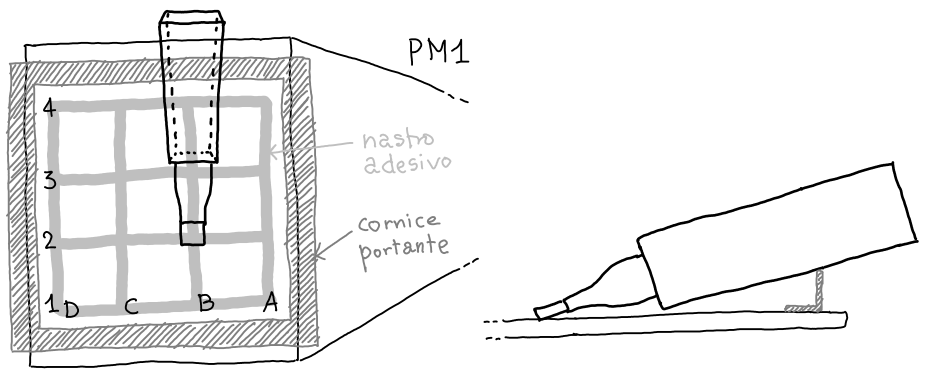
\includegraphics[width=\textwidth]{grigliaatt}
	\caption{\label{fig:grigliaatt}
	Apparato per la misura delle caratteristiche locali del PM1.
	Segnamo sul PM1 una griglia 4x4 di posizioni in cui mettere il miniscint.
	Le posizioni perimetrali (A1\dots4, D1\dots4, A\dots D1, A\dots D4)
	sono tali che il miniscint ha sempre la stessa inclinazione rispetto al PM1.}
\end{figure}

La possibilità di fare misure locali con il miniscint 
ci permette di misurare la lunghezza di attenuazione del sistema scintillatore più guida di luce. Avendo preso misure soltanto sullo scintillatore potrebbe sembrare che abbiamo misurato soltanto la sua lunghezza di attenuazione, ma la nostra strumentazione rivela un evento soltanto quando i fotoni rilasciati raggiungono il PMT dopo aver attraversato la guida di luce. 
Abbiamo eseguito le misure dividendo il PM1 in 16 caselle e ponendo su ognuna di esse il miniscint nei punti mostrati in \autoref{fig:grigliaatt}. 

Nel fare le misure sulle caselle perimetrali abbiamo appoggiato il miniscint sulla struttura che circonda il PM1 in modo che l'angolo tra esso ed il miniscint sia sempre lo stesso. Tale accorgimento ci permette di usare quelle misure per stimare l'efficienza locale relativa del PM1 che sarà trattata in \autoref{localis}.
Per ogni casella abbiamo acquisito il numero di coincidenze verificatesi in \SI{1000}{s}.
Al PM1 era collegata l'ADC in modo da poter registrare anche il rilascio di energia in ogni sezione.
Stimiamo che l'efficienza del PM1 fosse maggiore del \SI{50}\%.

Se chiamiamo $N$ il numero di raggi che attraversano ogni casella, possiamo legare questa quantità alla lunghezza di attenuazione attraverso la relazione \eqref{exp} in cui $x$ è la distanza orizzontale del miniscint dalla guida di luce; $N_0$ e $\lambda$ sono i parametri del fit. 
\begin{equation}
N=N_0 e^{-x/\lambda}  \label{exp}
\end{equation}

I dati raccolti sono stati trattati in due modi diversi perché entrambi permettono di ricavare la lunghezza di attenuazione e nessuno dei due ha delle caratteristiche che lo rendono preferibile rispetto all'altro.

\subsubsection{Media per colonne}

La prima strategia di analisi dati consiste nel fare la media dei conteggi per ognuna delle 4 colonne e poi fittare questi punti con la funzione \eqref{exp}.
Il fit ha restituito i seguenti risultati: $N_0=634\pm25$,  $\lambda=\SI{118\pm32}{cm}$, $\chi^2=11\pm2$ con dof=2 e correlazione corr$(N_0,\lambda)=-\SI{80}\%$. 
La \autoref{atte} mostra le medie ottenute e la relativa funzione di fit.
\marginpar{Togliere barre d'errore sulle $x$.}
\begin{figure}[h]
\centering
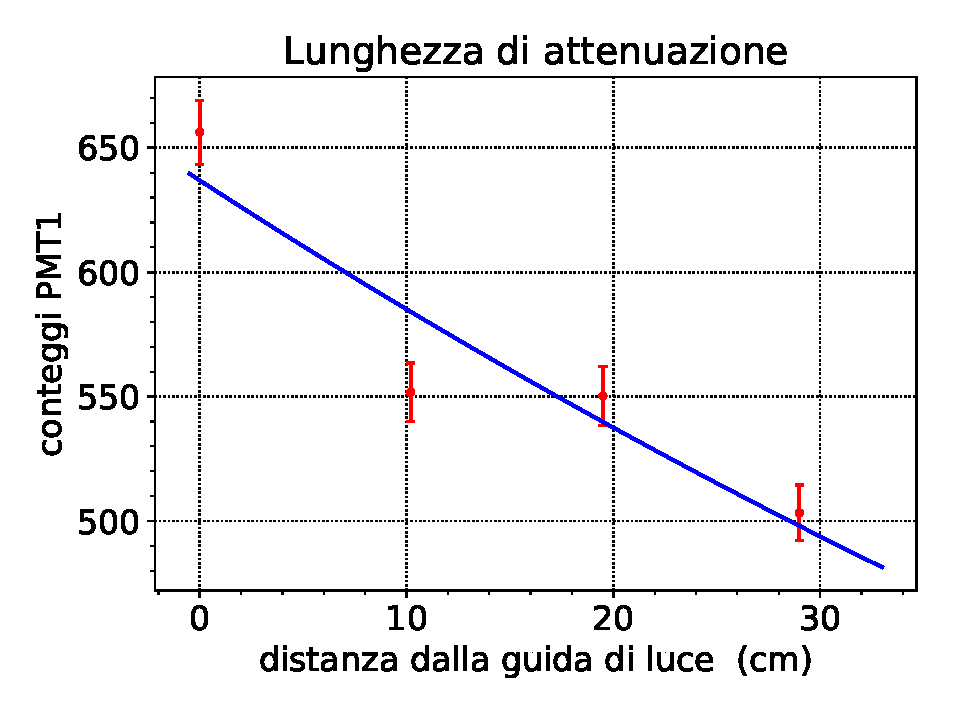
\includegraphics[width=8 cm]{atte}
\caption{Fit relativo alla lunghezza di attenuazione calcolata facendo la media per colonne.}
\label{atte}
\end{figure}

\begin{table}[h]
\centering
\begin{tabular}{| c | r @{$\pm$} l |}
\hline
colonna & \multicolumn{2}{c|}{media} \\
\hline
D & 503&11 \\
C & 550&12 \\
B & 551&12 \\
A & 656&13 \\
\hline
\end{tabular}
\caption{Dati del grafico in \autoref{atte}. La colonna D è quella più lontana dalla guida di luce.}
\end{table}

\subsubsection{Media per righe}

La seconda strategia adottata consiste nel fittare con la \eqref{exp} i conteggi di ogni riga separatamente e poi fare la media delle 4 lunghezze di attenuazione ottenute.
Le media sono state ottenute in questo modo: siano $\langle a \rangle$ il vettore che contiene la media dei parametri del fit e $V_i$ le matrici di covarianza dei 4 fit; sono legati dalla relazione 

\begin{equation*}
\langle a \rangle = \left(\sum{V_i^{-1}} \right)^{-1}  \left(\sum{V_i^{-1} a_i} \right).
\end{equation*}

La correlazione tra $\langle N_0 \rangle$ e $\langle \lambda \rangle$ è stata calcolata usando la matrice $W=\left(\sum{V_i^{-1}} \right)^{-1}$ attraverso la relazione
\begin{equation*}
\text{corr}(\langle N_0 \rangle ,\langle \lambda \rangle)=\frac{W_{A_0 \lambda}}{\sqrt{ W_{\lambda \lambda} W_{A_0 A_0}}}
\end{equation*}
in cui il nome dei parametri indica l'elemento opportuno di quella matrice.

In \autoref{4atte} è possibile vedere le 4 curve con le relative funzioni di fit, mentre la \autoref{tab:righe} contiene i risultati del fit.

\begin{table}[h]
\centering
\begin{tabular}{| c | r @{$\,\pm\,$} l  | r @{$\,\pm\,$} l  | c |}
\hline
riga & \multicolumn{2}{c|}{$N_0$} & \multicolumn{2}{c|}{ $\lambda$ [\si{cm}] } & $\chi^2$  \\
\hline
1 & 711&19 & 121&23 & 1  \\
2 & 638&32 & 127&47 & 4 \\
3 & 632&60 & 73&30 & 15 \\
4 & 565&21 & 228&111 & 2 \\
\hline
\end{tabular}
\caption{Risultati restituiti dai fit presenti in \autoref{4atte} riga per riga. Tutti i fit hanno 2 gradi di libertà e corr$(N_0,\lambda)=-0.8$. }
\label{tab:righe}
\end{table}


La media dei parametri dei fit restituisce $\langle\lambda\rangle=\SI{141\pm14}{cm}$, $\langle N_0\rangle=635\pm10$ e corr$(\langle N_0 \rangle ,\langle \lambda \rangle)=-0.66$.

\begin{figure}[h]
\centering
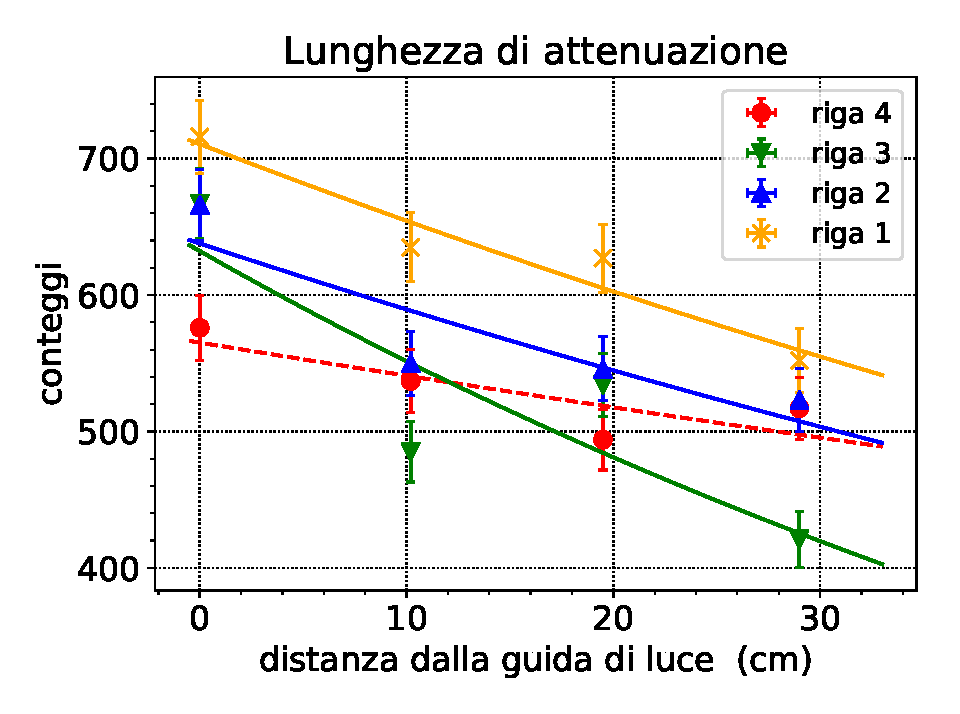
\includegraphics[width=8 cm]{4atte}
\caption{Fit relativo alla lunghezza di attenuazione calcolata facendo la media per righe. Il numero delle righe è quello indicato dalla \autoref{fig:grigliaatt}.}
\label{4atte}
\end{figure}


\subsubsection{Limiti della misura}

I parametri ricavati dai 2 fit precedenti sono compatibili ed hanno un errore maggiore del 10\%.
Con la strumentazione a nostra disposizione non è possibile determinare
la lunghezza di attenuazione con maggiore precisione.

Poiché il miniscint ha una dimensione significativa ($4\times4\times1\,\si{cm^3}$)
rispetto alle distanze in gioco (es. distanza dal bordo della lastra),
e non ha sempre la stessa inclinazione rispetto al PM1,
non è ben definito il punto del PM1 in cui facciamo una misura locale.

I fotoni, per arrivare al fotomoltiplicatore, non percorrono una linea retta,
ma vengono riflessi dal materiale che compone la lastra dello scintillatore e la guida di luce (riflessione totale)
oppure dalla carta argentata che riveste gli stessi.
Percorrendo queste traiettorie vengono attenuati ulteriormente e non abbiamo nessuna informazione
su come essi arrivino al PMT1 né in linea di massima né caso per caso.

\subsubsection{Lunghezza di attenuazione in energia.}

Abbiamo operato una media per colonne nello stesso modo visto prima, ma utilizzando i rilasci di energia misurati dall'ADC.
Dopo aver eseguito l'istogramma del rilascio di energia relativo a ciascuna delle 16 caselle,
abbiamo preso la moda delle occorrenze
e le abbiamo assegnato come errore la semilarghezza di quel canale dell'istogramma.
Poi abbiamo eseguito le medie sulle mode di ogni colonna.
Il grafico di \autoref{col} mostra l'inutilità di qualsivoglia fit esponenziale.

\begin{table}[h]
\centering
\begin{tabular}{| c | r @{$\,\pm\,$} l |}
\hline
colonna & \multicolumn{2}{c|}{media delle mode [mV]} \\
\hline
A & \qquad \quad 195&9 \\
B & 197&9 \\
C & 194&10 \\
D & 193&6 \\
\hline
\end{tabular}
\caption{Dati presenti in \autoref{col}.}
\label{tab:ADC}
\end {table}

\begin{figure}[h]
\centering
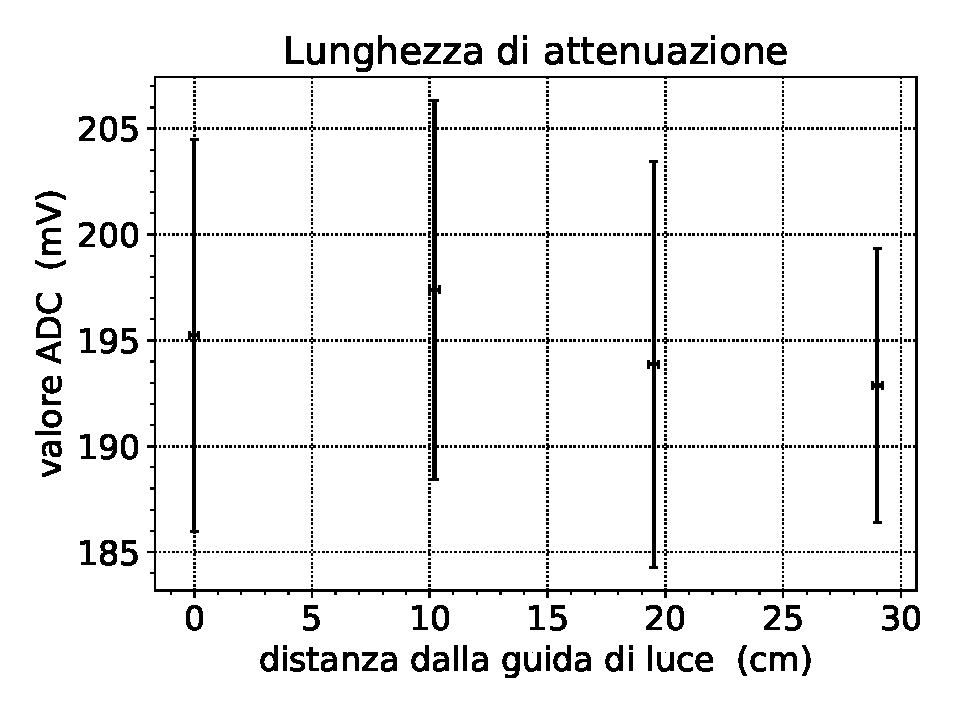
\includegraphics[width=8 cm]{ecol}
\caption{Energia media giunta al pmt per ogni colonna.}
\label{col}
\end{figure}


Anche questa volta abbiamo analizzato le singole righe, ma la \autoref{rig} mostra chiaramente quanto sia inutile tentare un fit con la funzione \eqref{exp}. 

\begin{figure}[h]
\centering
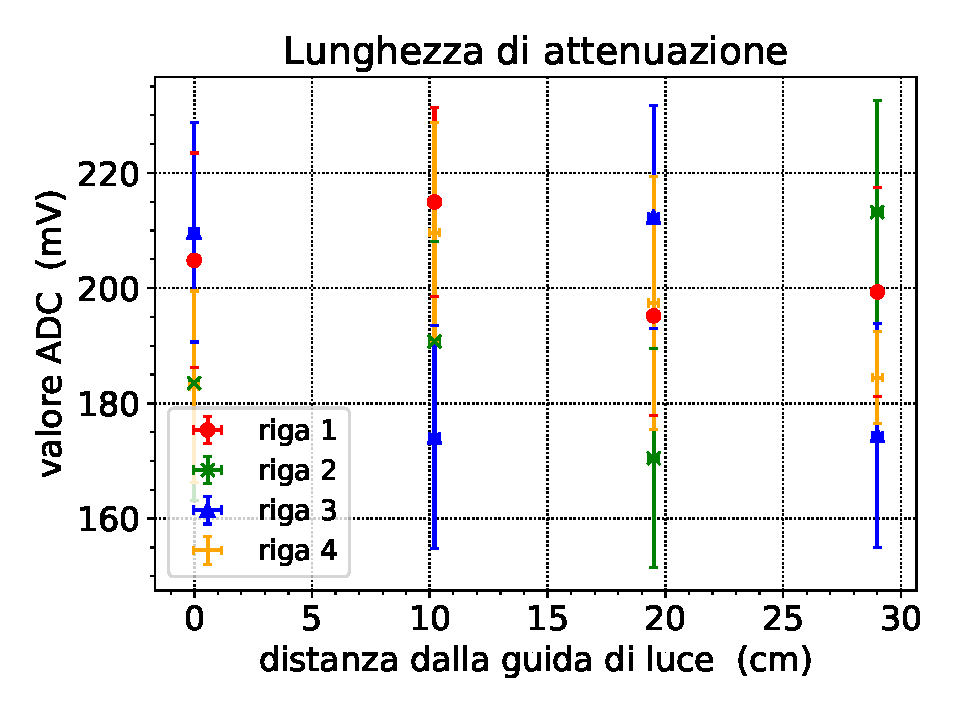
\includegraphics[width=8 cm]{erig}
\caption{Energia media giunta al pmt per ogni riga.
Ogni riga è stata sfasata leggermente rispetto alle altre per rendere leggibile la figura.}
\label{rig}
\end{figure}


